\documentclass[11pt, oneside]{article}   	% use "amsart" instead of "article" for AMSLaTeX format
\usepackage{geometry}                		% See geometry.pdf to learn the layout options. There are lots.
\geometry{letterpaper}                   		% ... or a4paper or a5paper or ... 
%\geometry{landscape}                		% Activate for rotated page geometry
%\usepackage[parfill]{parskip}    		% Activate to begin paragraphs with an empty line rather than an indent
\usepackage{graphicx}				% Use pdf, png, jpg, or eps§ with pdflatex; use eps in DVI mode
								% TeX will automatically convert eps --> pdf in pdflatex		
\usepackage{amssymb}

%SetFonts

%SetFonts

\title{Deep Learning}
\author{Bastien BRIER\\ bastien.brier@student.ecp.fr}
\date{December 6, 2016}				% Activate to display a given date or no date

\begin{document}
\maketitle
\vspace{-10pt}
\begin{center}
{\LARGE \bf Assignment 1}\\
\vspace{10pt}
\end{center}

\section{Data modelling: PCA and K-means}
\vspace{4pt}
	
	\subsection{PCA}
		We train our PCA algorithm on the training set, and we are asked to provide a plot of the error function :
		\[E(D)=\sum_{n\in Testset}\|I_n-\left(\sum\limits_{d=1}^Dc_{n,k}e_k+m\right)\|_2\]
		\begin{figure}[h]
			\centering
			\caption{Quality of the learned model\label{PCA}}
			\includegraphics[width=9.5cm]{/Users/bastienbrier/Pictures/PCA_error.png}
		\end{figure}
		
	\subsection{K-means}
		After having programmed the k-means algorithm, we evaluate the distortion criterion for k=2, and verify that it decreases as shown in the graphics below.
		\begin{figure}[h]
			\centering
			\caption{Decrease of the distortion criterion \label{K-means}}
			\includegraphics[width=9.5cm]{/Users/bastienbrier/Pictures/K-means_iteration.png}
		\end{figure}
		\\We then perform the algorithm ten times and keep the solution that minimises the distortion. Here are the resulting digit clusters.
		\begin{figure}[h]
			\centering
			\caption{Digit clusters \label{K-means}}
			\includegraphics[width=9.5cm]{/Users/bastienbrier/Pictures/K-means_clusters.png}
		\end{figure}
		\\ Finally, we repeat the procedure for k = 3,4,5,10,50,100 and observe that the cost	decreases as k increases, as shown below.
		\\ We computed the cost of the k-means algorithm according to this formula ($c_n$ being the centroid to which $I_n$ was affected) :
		\[E(k)=\sum_{n\in Testset}\|I_n-c_n\|_2\]
		\begin{figure}[h]
			\centering
			\caption{Decrease of the k-means distortion cost \label{K-means}}
			\includegraphics[width=9.5cm]{/Users/bastienbrier/Pictures/K-means_error.png}
		\end{figure}
		\\ PCA and K-means perform similarly on train set data (from $1.8\times10^4$ to $1.2\times10^4$), but the PCA generalises better on unseen data. This difference can be 		explained because PCA is a dimensionality reduction technique whereas k-means is a clustering algorithm. In order to mitigate this error, a good practice could be to 			combine both techniques.
		
\vspace{4pt}	
\section{Ising model: MCMC and learning}
\vspace{4pt}
	
	\subsection{Part-1: Brute-force evaluations}
		In this exercise, we consider an Ising model based on a 4x4 lattice. We first consider exhaustively all $2(N^2)$ states, energies and associated probabilities. The energy 			is of the form:
		\[E(\mathbf x;J)=\sum_{(i,j)\in\mathcal E}x_ix_j=-\frac{J}{2}\mathbf x^T\mathbf A\mathbf x\] 
		where $J$ is a scalar and $\mathcal E$ is the set of edges of a rectangular grid, $\mathbf A$ is the 16x16 incidence matrix of the network.
		\\ We then compute the partition function:
		\[Z=\sum_\mathbf x\exp(-E(\mathbf x;J))\] 
		\\ As shown below, the probability that the network is in any state $\mathbf x$ is given by:
		\[P(\mathbf x;J)=\frac{1}{Z}\exp(-E(\mathbf x;J))\] 
		\begin{figure}[h]
			\centering
			\caption{Probabilities of each state\label{pstate}}
			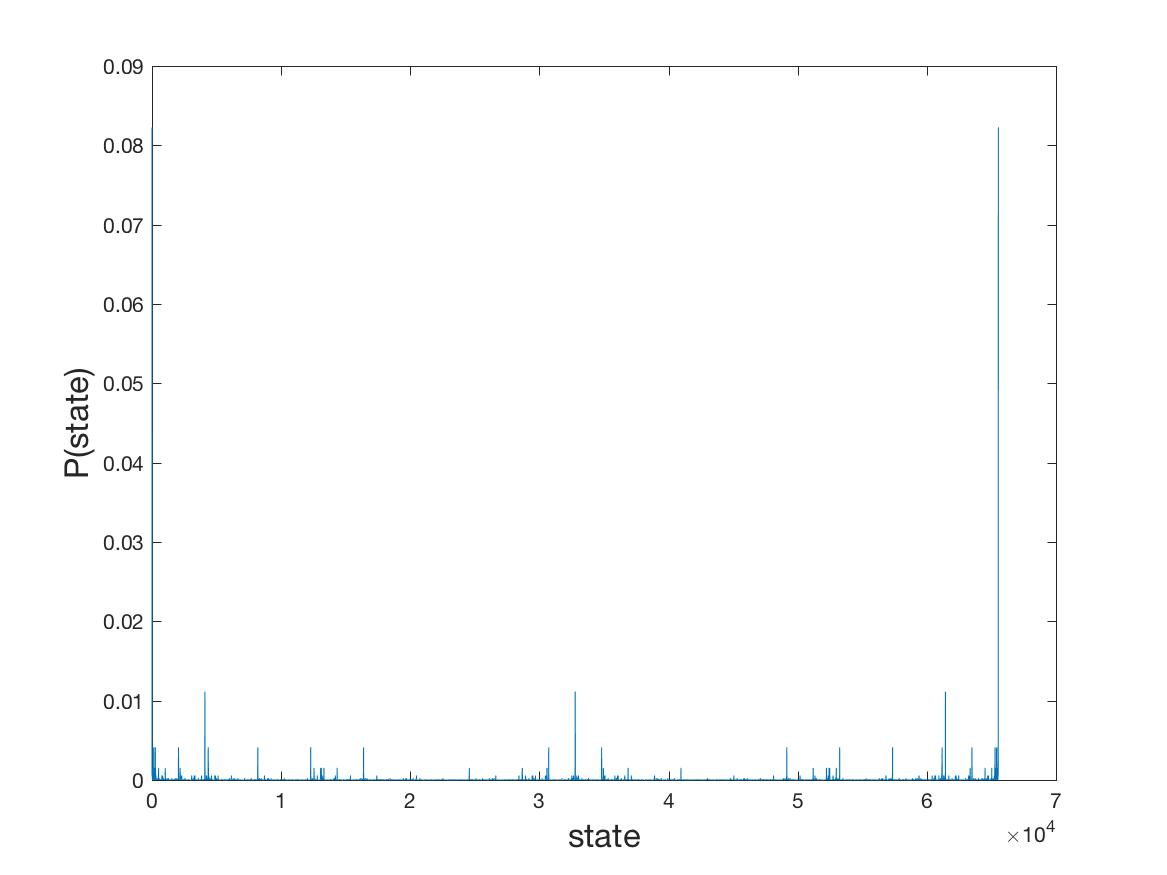
\includegraphics[width=9.5cm]{/Users/bastienbrier/Pictures/pstate.jpg}
		\end{figure}
		\\ And, for all features $\phi_k(x), k = 1,. . .,K$, we compute their expectations under the model:
		\[E^{PJ}_k= \langle\phi_k(\mathbf x)\rangle_{P(\mathbf x;J)} = \sum_\mathbf xP(\mathbf x;J)\phi_k(\mathbf x)\]
		\\ In figure 6, we can see the result of the calculation of this expectation.
		\begin{figure}[h]
			\centering
			\caption{Features expectations\label{expectations}}
			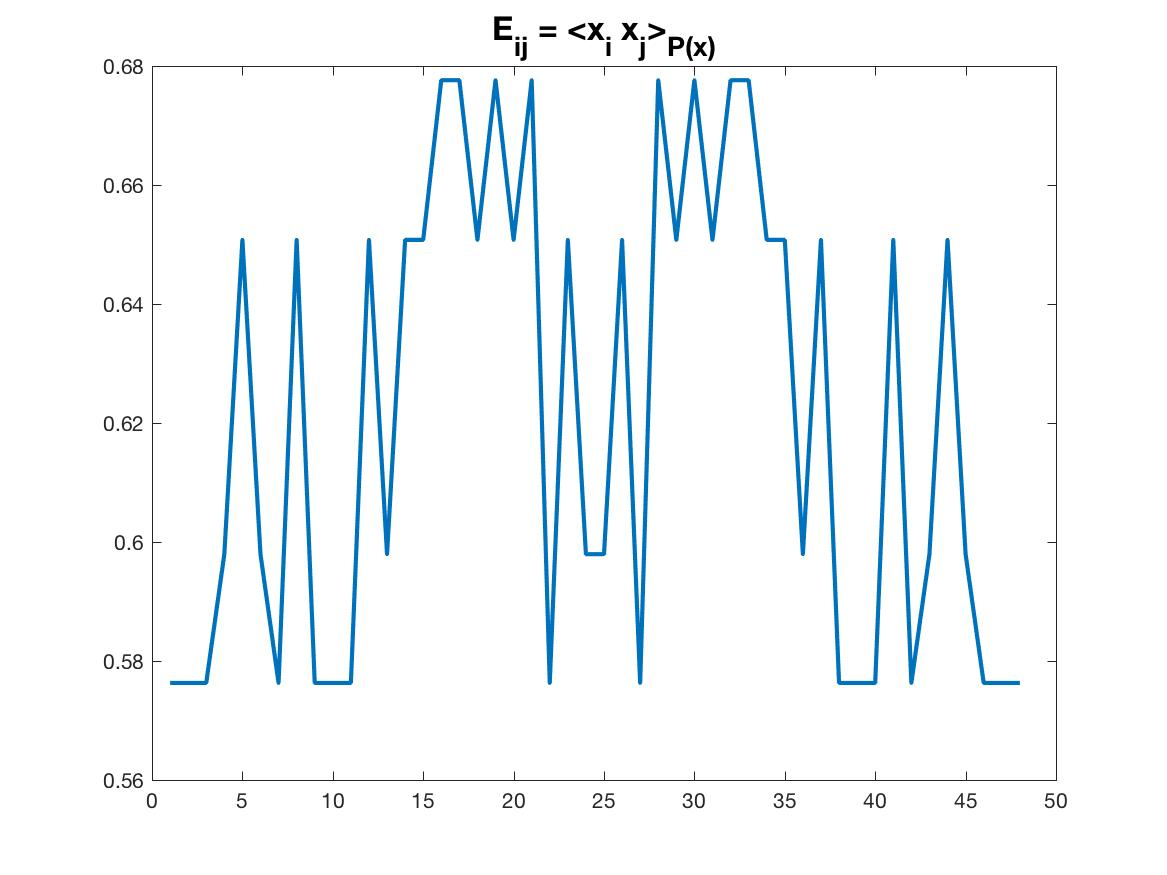
\includegraphics[width=8cm]{/Users/bastienbrier/Pictures/Expectations.jpg}
		\end{figure}
		\vspace{150pt}	
		
	\subsection{Part-2: MCMC evaluations}
		We use Gibbs sampling to obtain Monte Carlo estimates of the quantities computed in the previous subsection:
		\[E_k^{MC}(N)=\sum_{n=1}^N\phi_k(\mathbf x_n)\]
		\begin{figure}[h]
			\centering
			\caption{Progression of Monte Carlo estimates and Comparison between Monte Carlo and Brute Force}
			\begin{tabular}{cc}
				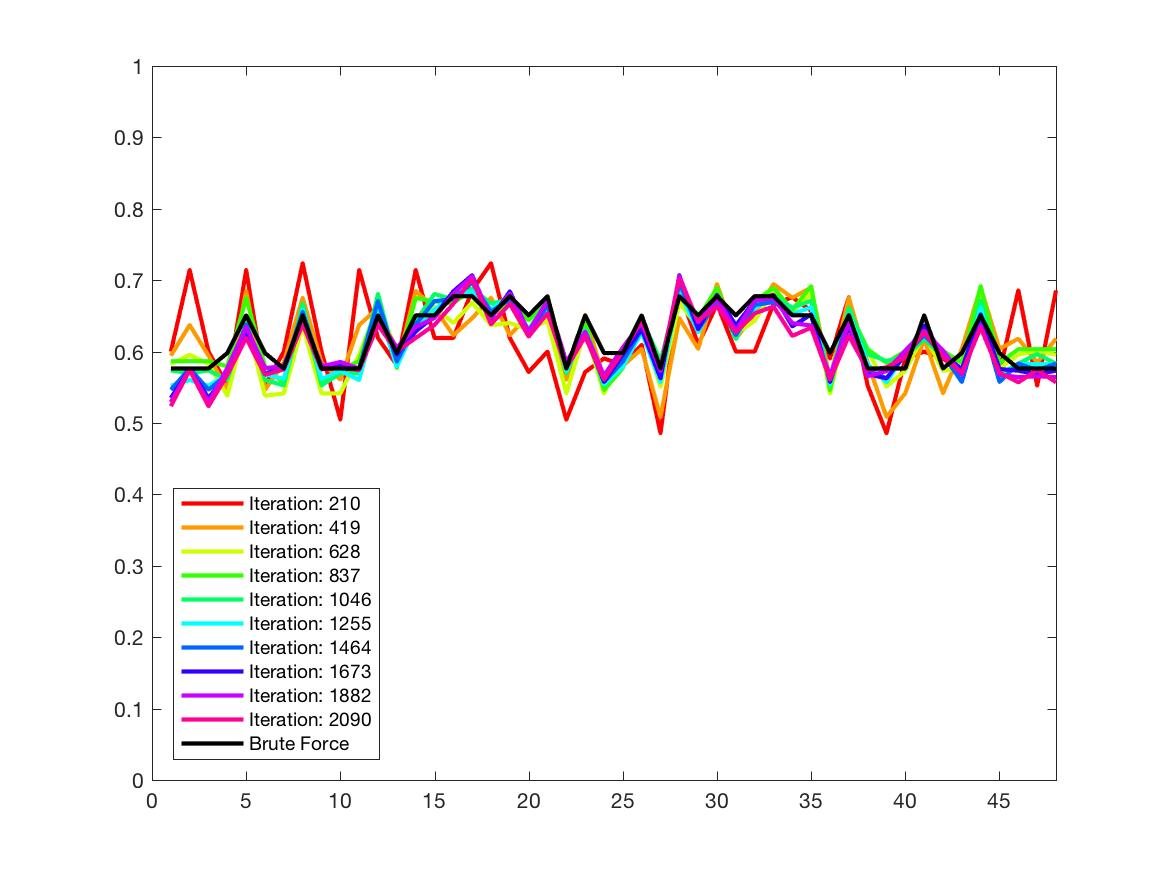
\includegraphics[width=8cm]{/Users/bastienbrier/Pictures/Estimates.jpg}
				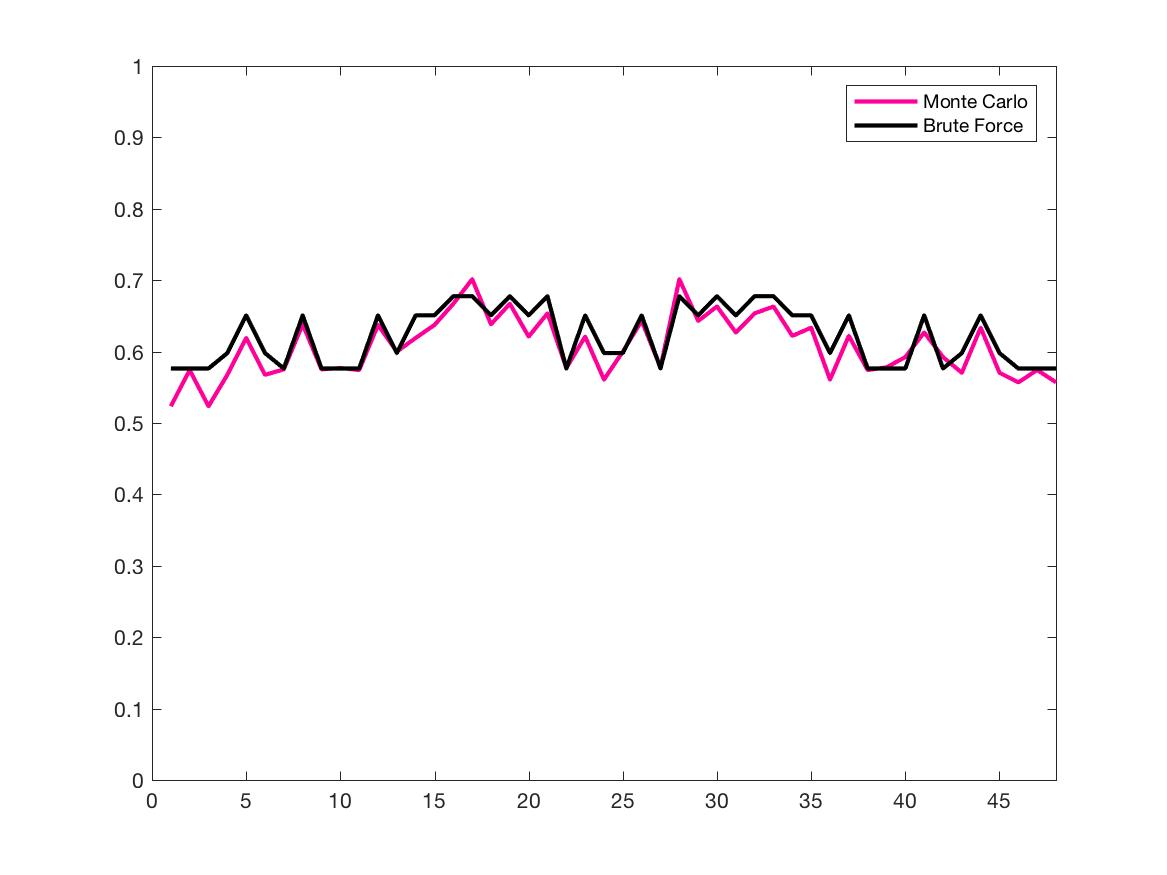
\includegraphics[width=8cm]{/Users/bastienbrier/Pictures/MCvsBF.jpg}
			\end{tabular}
		\end{figure}
	
	\subsection{Part-3: Parameter Estimation}
		In this part, we want to estimate the value of $J$ that is most likely to be responsible for the values of $E^{PJ}$. In other words, we try to find the maximum likelihood estimate of $J$. We seek therefore to maximise the log-likelihood of J, which can be expressed:
		\[log(L(x_1, ... , x_n;J))= -NlogZ - \sum_nE(x_n;J)\]
		\\ This value is maximum for $\frac{\partial log(L(x_1, ... , x_n;J))}{\partial J} = 0$. As we observe that the Ising model described is a member of the exponential family, this value is obtained for:
		\[\langle \phi_k\rangle_{emp} = \langle \phi_k\rangle_{P(\mathbf x;J)}\]
		\\ We use a gradient ascent technique to find a global maximum with this formula:
		\[J = J - \delta (\langle \phi_k\rangle_{emp} - \langle \phi_k\rangle_{P(\mathbf x;J)})\]
		\\ $\delta$ is the step we use to update J. After some experiments, a value of $\delta = 0.015$ is the one which yields the most precise result. We then find a value of $J = 0.6986$.
		\begin{figure}[h]
			\centering
			\caption{Estimation of J by gradient ascent\label{gradient}}
			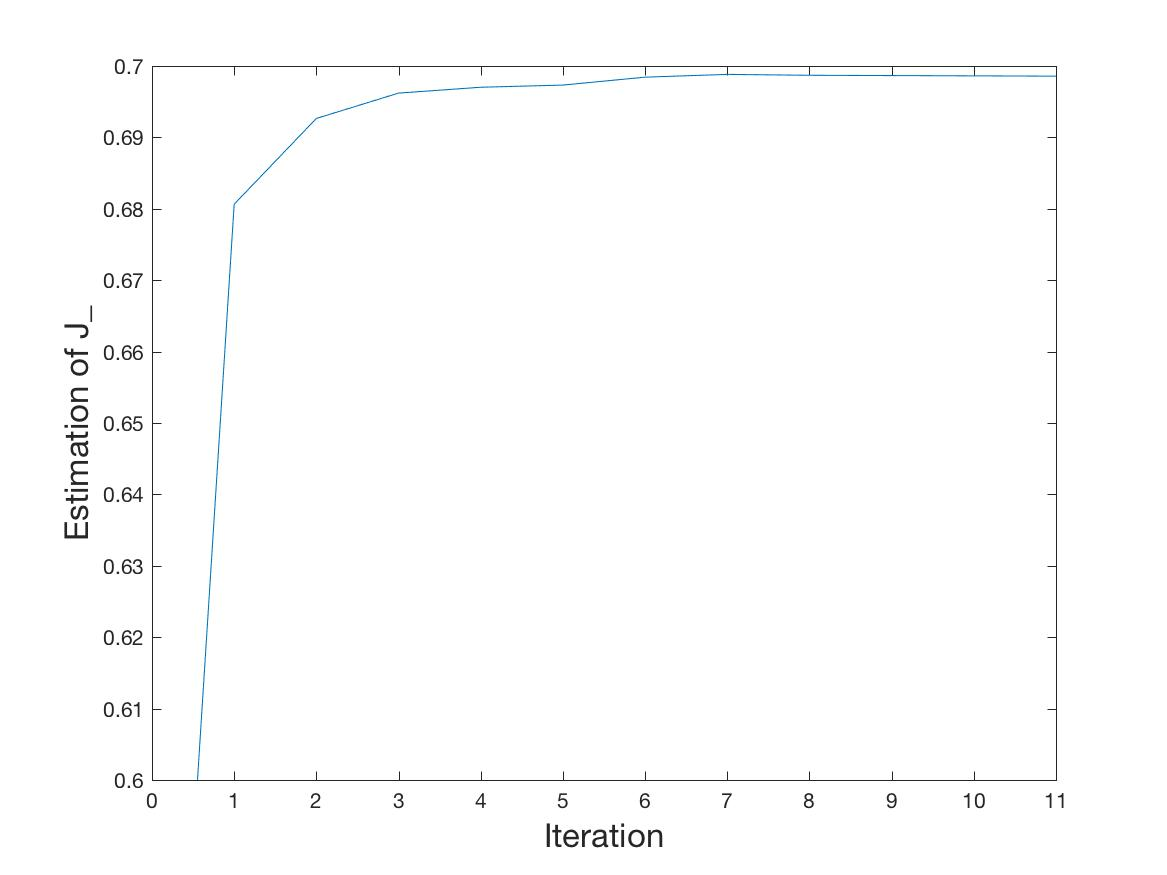
\includegraphics[width=10cm]{/Users/bastienbrier/Pictures/J.jpg}
		\end{figure}
		\\ We then plot the expectations.
		\makeatletter
		\setlength{\@fptop}{0pt}
		\makeatother
		\begin{figure}[t!]
			\centering
			\caption{Progression of the estimation per iteration and Comparison between estimated and desired models}
			\begin{tabular}[t!]{cc}
				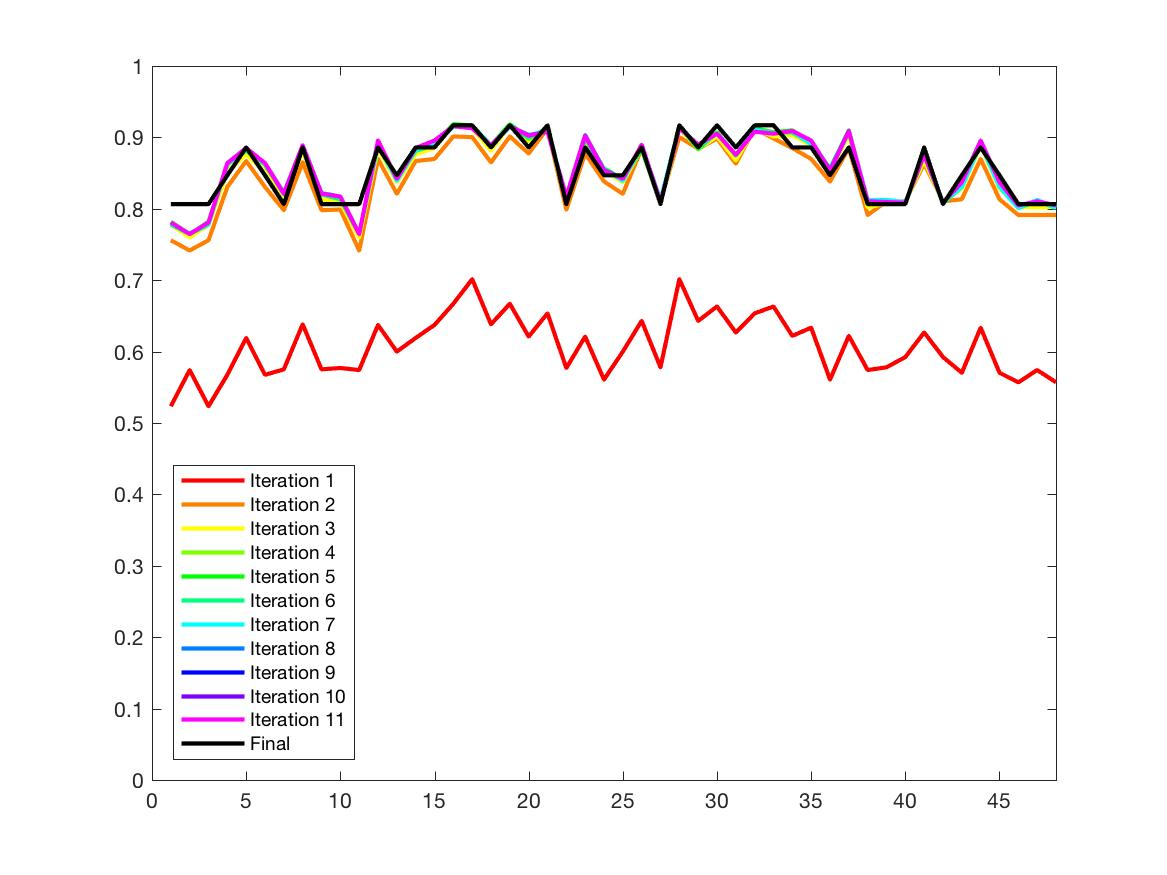
\includegraphics[width=8cm]{/Users/bastienbrier/Pictures/updates.jpg}
				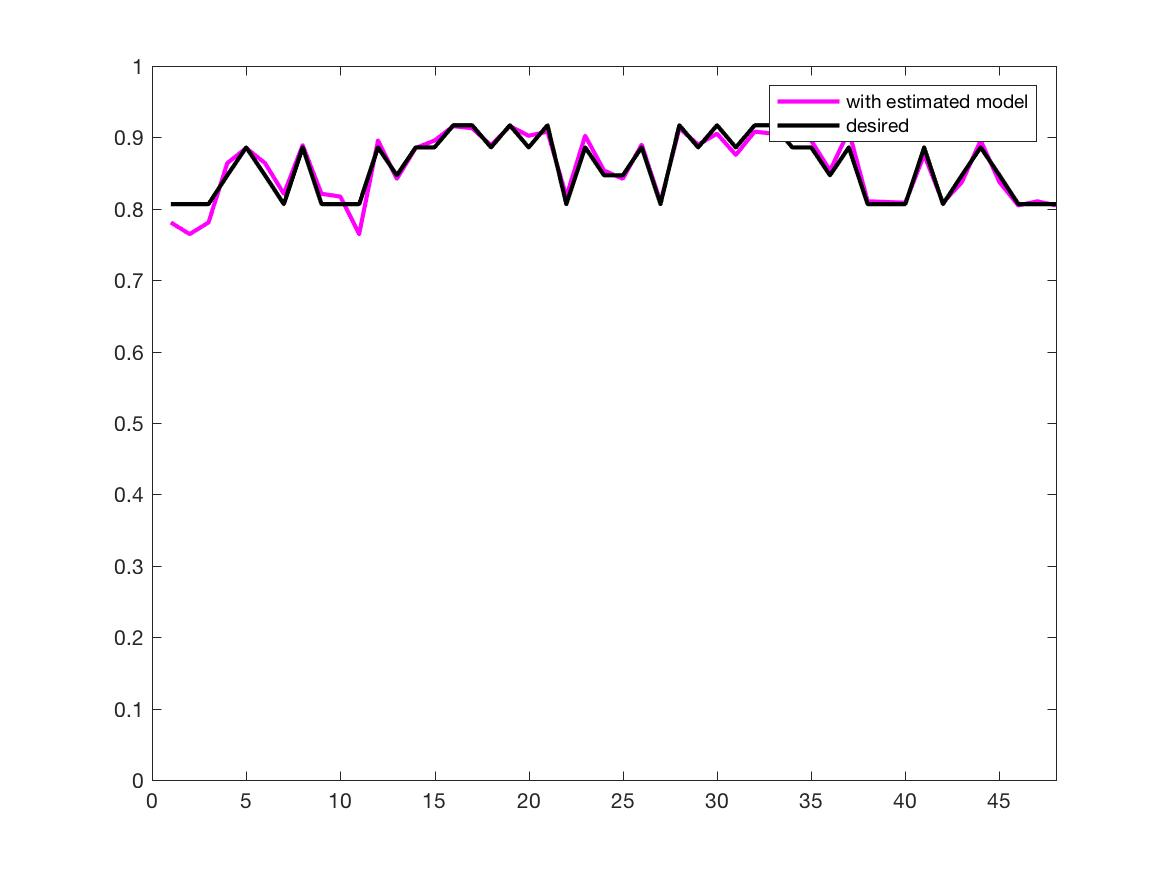
\includegraphics[width=8cm]{/Users/bastienbrier/Pictures/final.jpg}
			\end{tabular}
		\end{figure}
	
\end{document}  